\documentclass[aspectratio=169]{beamer}

% --- THEME AND STYLING ---
\usetheme{Madrid}
\useoutertheme{default}
\useinnertheme{rectangles}
\setbeamertemplate{navigation symbols}{}

% --- CUSTOM COLOR PALETTE ---
\definecolor{SkyBlue}{RGB}{135, 206, 235}
\definecolor{DarkNavy}{RGB}{0, 0, 139}
\definecolor{LightBlueBg}{RGB}{240, 248, 255}
\definecolor{AccentBlue}{RGB}{70, 130, 180}
\definecolor{DarkGreyText}{RGB}{50, 50, 50}
\definecolor{HighlightGreen}{RGB}{34, 139, 34}
\definecolor{AlertRed}{RGB}{220, 20, 60}

\setbeamercolor{palette primary}{bg=SkyBlue,fg=DarkNavy}
\setbeamercolor{palette secondary}{bg=DarkNavy,fg=white}
\setbeamercolor{palette tertiary}{bg=AccentBlue,fg=white}
\setbeamercolor{palette quaternary}{bg=SkyBlue,fg=DarkNavy}
\setbeamercolor{structure}{fg=DarkNavy}
\setbeamercolor{section in toc}{fg=DarkNavy}
\setbeamercolor{frametitle}{bg=SkyBlue,fg=DarkNavy}
\setbeamercolor{block title}{bg=DarkNavy,fg=white}
\setbeamercolor{block body}{bg=LightBlueBg,fg=DarkGreyText}
\setbeamercolor{block title alerted}{bg=AlertRed,fg=white}
\setbeamercolor{block body alerted}{bg=LightBlueBg,fg=DarkGreyText}
\setbeamercolor{block title example}{bg=HighlightGreen,fg=white}
\setbeamercolor{block body example}{bg=LightBlueBg,fg=DarkGreyText}
\setbeamertemplate{footline}[frame number]
\setbeamercolor{footline}{fg=DarkNavy}
\setbeamertemplate{blocks}[rounded][shadow=false]

% --- PACKAGES ---
\usepackage[utf8]{inputenc}
\usepackage{amsmath,amssymb}
\usepackage{booktabs}
\usepackage{graphicx}
\usepackage{array}
\usepackage{multirow}
\usepackage{tikz}
\usepackage{siunitx}

% --- TITLE PAGE ---
\title[Sustainable Rendezvous]{Sustainable "Rendezvous": A Festival Systems Challenge}
\subtitle{Comprehensive Process Optimization (Modules 3.1 - 3.4)}
\author[Team Sustainability]{Sustainability Task Force}
\institute{Department of Chemical Engineering\\
\vspace{0.2cm}
\small Course: CLL782 - Process Optimization\\
\small Instructor: Prof. Om Prakash}
\date{\today}

\begin{document}

% --- TITLE SLIDE ---
\begin{frame}[plain]
    \titlepage
    \vspace{-0.5cm}
    \begin{center}
        \small Presented by: Yash
    \end{center}
\end{frame}

% --- OUTLINE ---
\begin{frame}{Outline}
    \tableofcontents[hideallsubsections]
\end{frame}

%%%%%%%%%%%%%%%%%%%%%%%%%%%%%%%%%%%%%%%%%%%%%%%%%%%%%%%%%%%%%%%%%
\section{1. The Genesis \& Vision}
%%%%%%%%%%%%%%%%%%%%%%%%%%%%%%%%%%%%%%%%%%%%%%%%%%%%%%%%%%%%%%%%%

\begin{frame}{The Genesis: From Biodiversity to Urban Chaos}
    \begin{columns}[T]
        \begin{column}{0.6\textwidth}
            \begin{block}{The Inspiration}
                Sanskruti, General Secretary (Cultural Affairs), hails from the biodiverse landscapes of West Champaran.
                \begin{itemize}
                    \item \textbf{Observation}: Urban life offers convenience but at a massive, silent environmental cost.
                    \item \textbf{The Trigger}: "Rendezvous" (Asia's Largest Fest) generates tons of waste, acting as a microcosm of this urban un-sustainability.
                \end{itemize}
            \end{block}
            
            \begin{alertblock}{The Vision}
                \textit{"Sustainability is not about restriction, but about acting responsibly and optimizing resources."}
                
                Transform Rendezvous from a logistical challenge into a \textbf{Model of Sustainability}.
            \end{alertblock}
        \end{column}
        
        \begin{column}{0.35\textwidth}
            \begin{exampleblock}{The Objective}
                Use \textbf{Systems Engineering \& Optimization} to:
                \begin{enumerate}
                    \item Quantify Impact.
                    \item Optimize Infrastructure.
                    \item Minimize Waste.
                \end{enumerate}
            \end{exampleblock}
        \end{column}
    \end{columns}
\end{frame}

\begin{frame}{Scope: The High-Intensity Zone}
    \begin{columns}[T]
        \begin{column}{0.55\textwidth}
            To ensure impact, we focus on the festival's core activity hub.
            
            \begin{table}
                \centering\small
                \begin{tabular}{l l}
                    \toprule
                    \textbf{Parameter} & \textbf{Value} \\ \midrule
                    \textbf{Total Campus} & 320 Acres \\
                    \textbf{Target ROI Area} & \textbf{82 Acres} (26\%) \\
                    \textbf{Key Venues} & OAT, Nalanda, SAC, LHC \\
                    \textbf{Peak Footfall} & $\sim$40,000 / day \\
                    \textbf{Grid System} & 137 Cells (0.6 acres each) \\
                    \bottomrule
                \end{tabular}
            \end{table}
        \end{column}
        \begin{column}{0.40\textwidth}
            \centering
             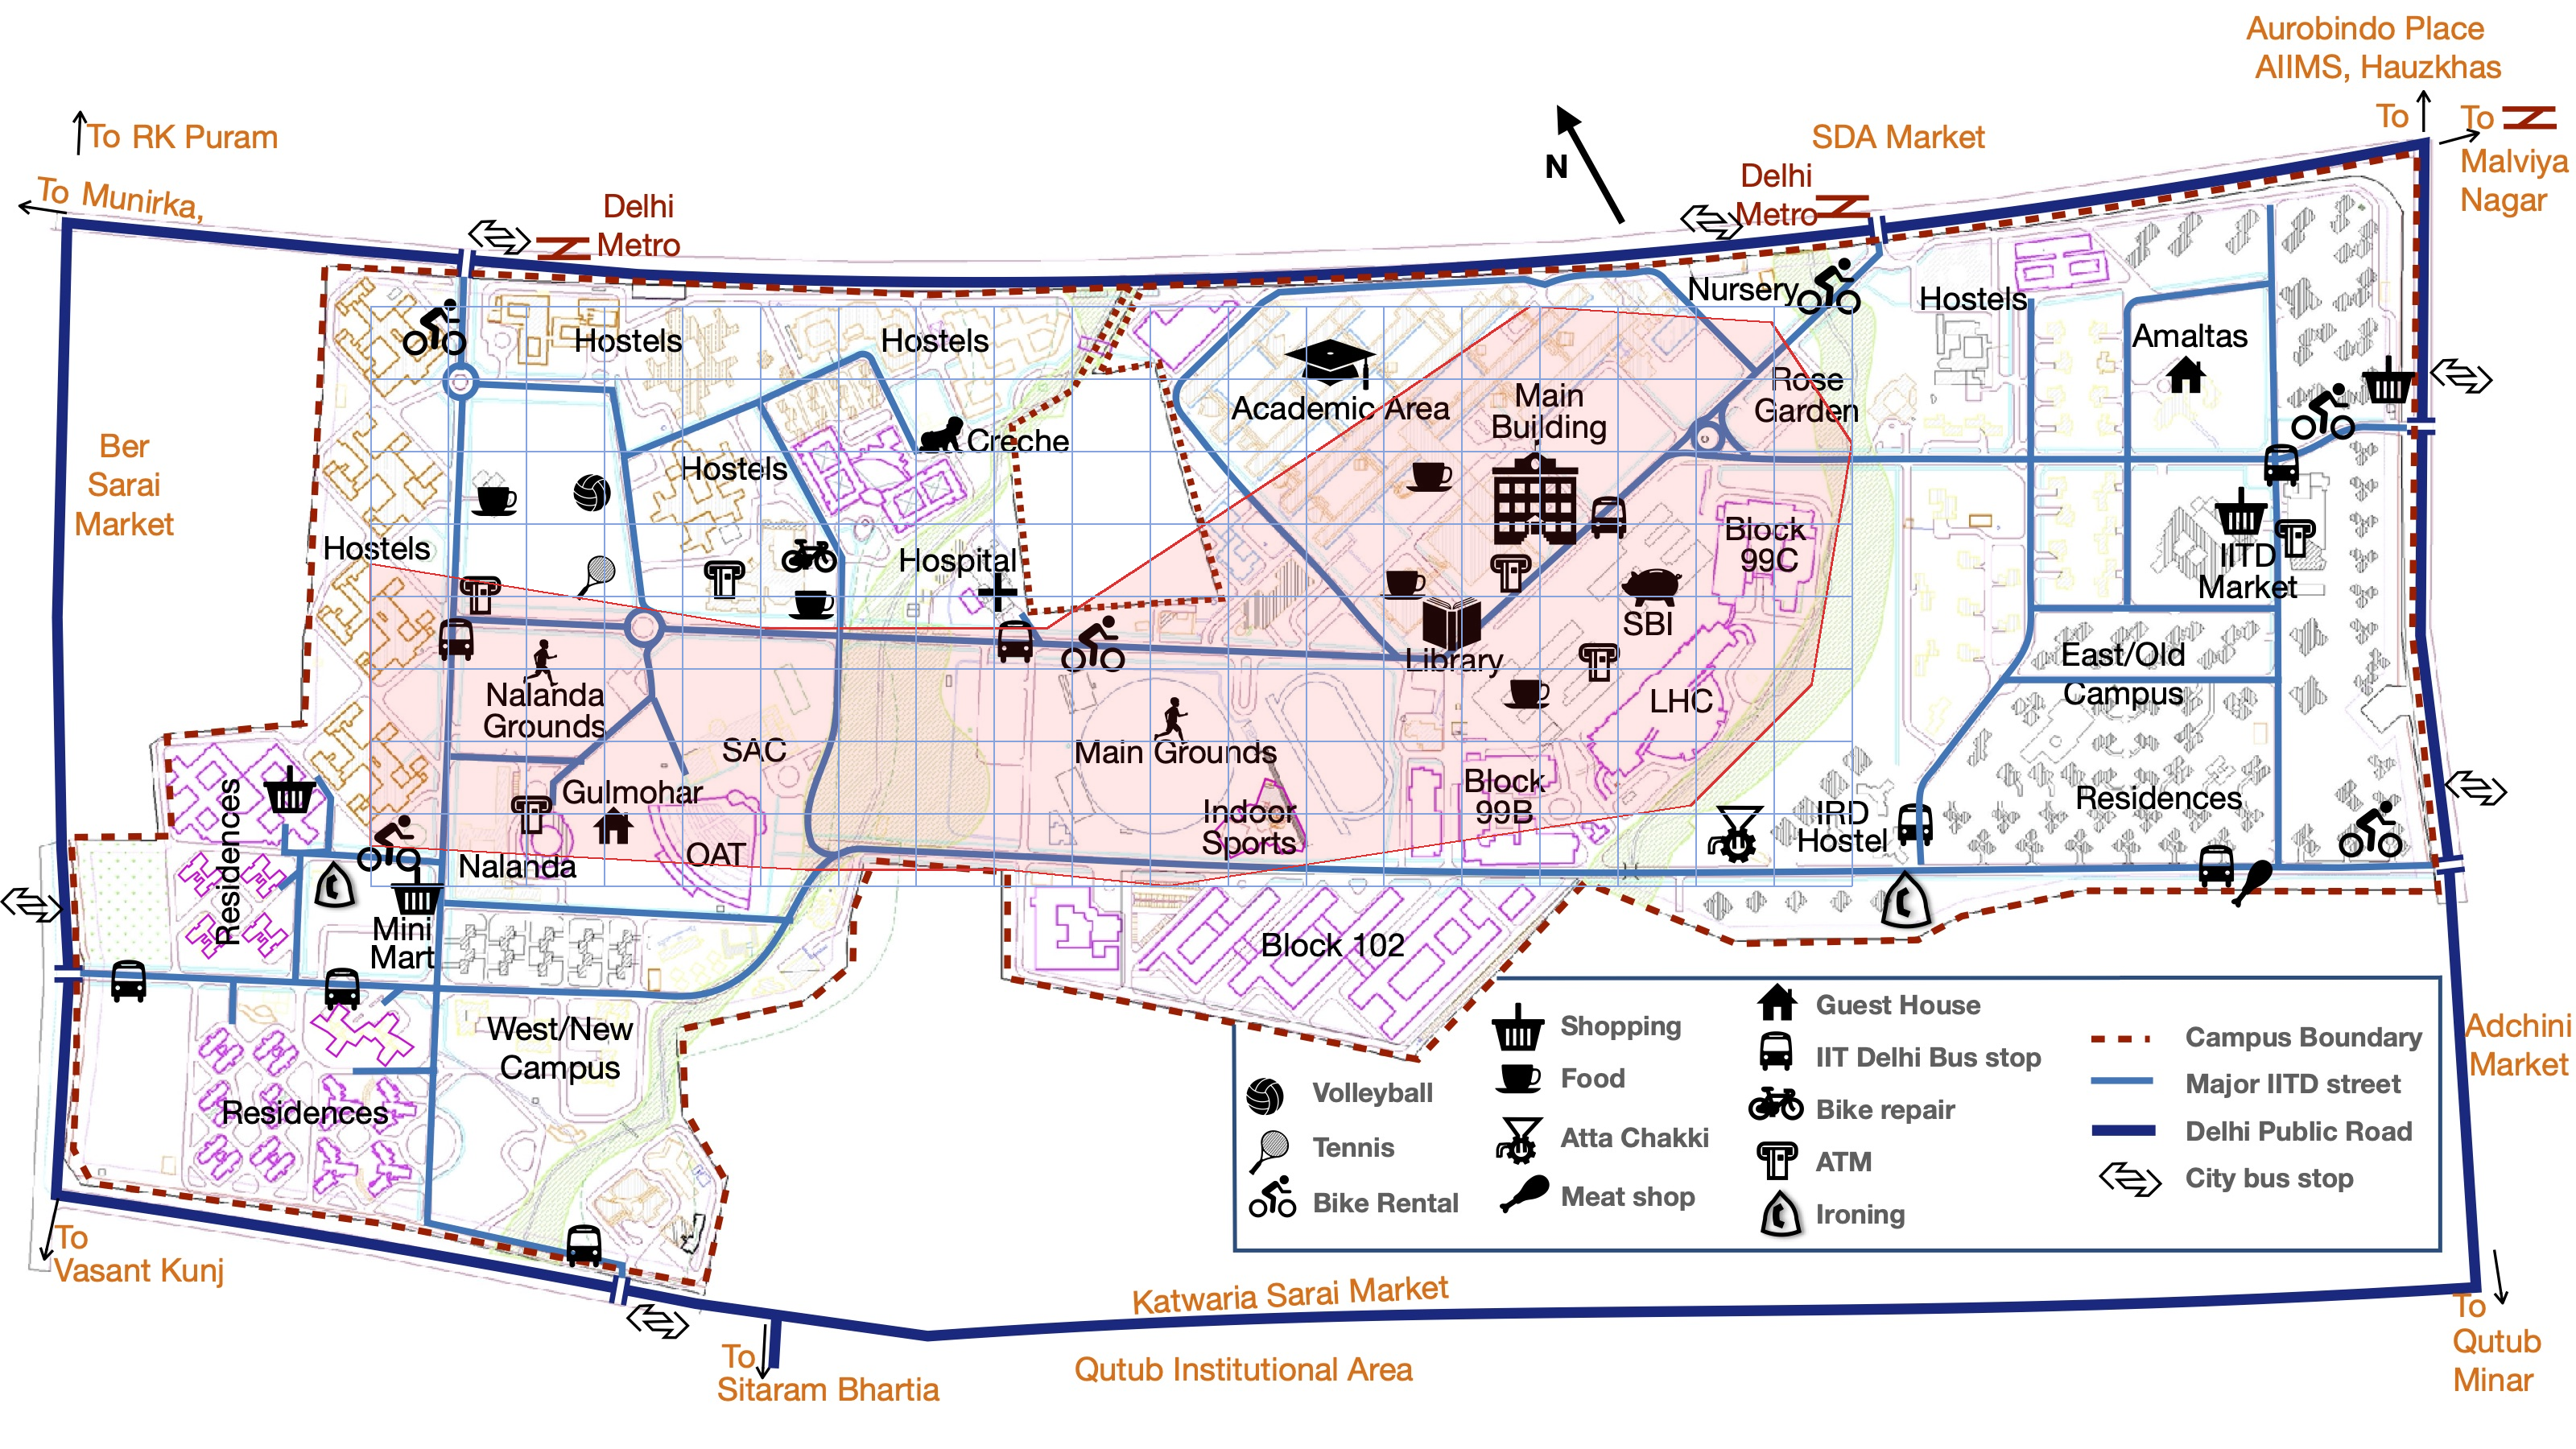
\includegraphics[width=0.95\textwidth]{../Module_3_1/iitd_roi_grid_map.jpg} \\
             \tiny{Figure: ROI with 137 Grid Cells}
        \end{column}
    \end{columns}
\end{frame}

%%%%%%%%%%%%%%%%%%%%%%%%%%%%%%%%%%%%%%%%%%%%%%%%%%%%%%%%%%%%%%%%%
\section{2. Module 3.1: Environmental Load}
%%%%%%%%%%%%%%%%%%%%%%%%%%%%%%%%%%%%%%%%%%%%%%%%%%%%%%%%%%%%%%%%%

\begin{frame}{3.1 Problem Statement \& Variables}
    \textbf{Problem:} Develop a mathematical function $E(N, S, A)$ to quantify total environmental load, capturing non-linear "crowding" and "congestion" effects.

    \vspace{0.2cm}
    \begin{table}
        \caption{Module 3.1 Variable Definitions}
        \centering\footnotesize
        \begin{tabular}{l l l l}
            \toprule
            \textbf{Sym} & \textbf{Description} & \textbf{Unit} & \textbf{Type} \\ \midrule
            $N$ & Number of Attendees & Persons & Parameter (Demand) \\
            $S$ & Number of Food Stalls & Stalls & \textbf{Decision Variable} \\
            $A$ & Activity Duration & Hours & Decision Variable \\
            $\alpha_2$ & Stall Embodied Impact & kg CO$_2$/stall & Constant (18.0) \\
            $\gamma_{NS}$ & Congestion Penalty & - & Constant (0.0005) \\
            $E$ & \textbf{Total Env Load} & kg CO$_2$-eq & \textbf{Objective} \\
            \bottomrule
        \end{tabular}
    \end{table}
\end{frame}

\begin{frame}{3.1 Formulation \& Insights}
    \begin{alertblock}{Objective Function}
        $$ E = \underbrace{(\alpha_1 N + \alpha_2 S)}_{\text{Base Load}} + \underbrace{(\beta_N N^{1.3})}_{\text{Non-linear Scale}} + \underbrace{\left( \gamma_{NS} \frac{N^2}{S} \right)}_{\text{Congestion Penalty}} $$
    \end{alertblock}

    \begin{itemize}
        \item \textbf{Trade-off}: 
            \begin{itemize}
                \item Too few stalls ($S \downarrow$) $\rightarrow$ High Congestion ($N^2/S \uparrow$) $\rightarrow$ Littering.
                \item Too many stalls ($S \uparrow$) $\rightarrow$ High Embodied Energy ($\alpha_2 S \uparrow$).
            \end{itemize}
        \item \textbf{Analytical Solution}:
            $$ \frac{dE}{dS} = \alpha_2 - \gamma_{NS} \frac{N^2}{S^2} = 0 \implies S^* = N \sqrt{\frac{\gamma_{NS}}{\alpha_2}} $$
        \item \textbf{Result}: For $N=40,000$, $S^* \approx \textbf{210 Stalls}$. (Current practice is suboptimal).
    \end{itemize}
\end{frame}

%%%%%%%%%%%%%%%%%%%%%%%%%%%%%%%%%%%%%%%%%%%%%%%%%%%%%%%%%%%%%%%%%
\section{3. Module 3.2: Dustbin Placement (FLP)}
%%%%%%%%%%%%%%%%%%%%%%%%%%%%%%%%%%%%%%%%%%%%%%%%%%%%%%%%%%%%%%%%%

\begin{frame}{3.2 Problem Statement \& Variables}
    \textbf{Problem:} Optimally place dustbins ($j$) to cover demand zones ($i$) such that walking distance is minimized, subject to service radius ($R_t$).

    \vspace{0.2cm}
    \begin{table}
        \centering\footnotesize
        \begin{tabular}{l l l l}
            \toprule
            \textbf{Sym} & \textbf{Description} & \textbf{Unit} & \textbf{Type} \\ \midrule
            $i$ & Index of Demand Zone & - & Index ($1 \dots 137$) \\
            $j$ & Candidate Location & - & Index \\
            $y_{j,t}$ & Install Bin type $t$ at $j$? & $\{0,1\}$ & \textbf{Binary Decision} \\
            $a_{i,j,t}$ & Fraction demand $i \to j$& $[0,1]$ & Continuous Decision \\
            $F_i$ & Footfall at Zone $i$ & Ppl/hr & Parameter \\
            $R_t$ & Service Radius & m & Const (30-50m) \\
            $K_t$ & Bin Capacity & kg & Const (30kg) \\
            \bottomrule
        \end{tabular}
    \end{table}
\end{frame}

\begin{frame}{3.2 Mathematical Formulation}
    \begin{exampleblock}{Minimize User Inconvenience (Weighted Distance)}
        $$ \text{Min } Z = \sum_{i} \sum_{j} \sum_{t} \left( F_i \cdot a_{i,j,t} \cdot D_{ij} \right) $$
    \end{exampleblock}

    \textbf{Subject to Constraints:}
    \vspace{0.2cm}
    \begin{enumerate}
        \item \textbf{Coverage Requirement}: $\sum_{j,t} a_{i,j,t} = 1 \quad \forall i$
        \item \textbf{Capacity Limit}: $\sum_{i} (F_i \cdot w \cdot a_{i,j,t}) \le K_t \cdot y_{j,t} \quad \forall j,t$
        \item \textbf{Service Radius}: $a_{i,j,t} = 0 \quad \text{if } D_{ij} > R_t$
        \item \textbf{Logical Link}: $a_{i,j,t} \le y_{j,t}$
    \end{enumerate}
\end{frame}

%%%%%%%%%%%%%%%%%%%%%%%%%%%%%%%%%%%%%%%%%%%%%%%%%%%%%%%%%%%%%%%%%
\section{4. Module 3.3: Waste Logistics}
%%%%%%%%%%%%%%%%%%%%%%%%%%%%%%%%%%%%%%%%%%%%%%%%%%%%%%%%%%%%%%%%%

\begin{frame}{3.3 Problem Statement \& Variables}
    \textbf{Problem:} Design a logistics network to clear 6 tons of waste/day using a fleet of vehicle ($k$) from zones ($i$) to facilities ($j$).

    \vspace{0.2cm}
    \begin{table}
        \centering\footnotesize
        \begin{tabular}{l l l l}
            \toprule
            \textbf{Sym} & \textbf{Description} & \textbf{Unit} & \textbf{Type} \\ \midrule
            $x_{i,j}$ & Waste Flow $i \to j$ & kg & \textbf{Continuous Decision} \\
            $v_k$ & Vehicle $k$ Deployed? & $\{0,1\}$ & Binary Decision \\
            $V_{cap}$ & Vehicle Payload & kg & Const (750 kg) \\
            $C_{dist}$ & Transport Cost & Rs/km & Const (Rs. 20) \\
            $C_{proc}$ & Processing Cost & Rs/kg & Const (Facility dep.) \\
            $C_{fix}$ & Vehicle Fixed Cost & Rs/day & Const (Rs. 800) \\
            \bottomrule
        \end{tabular}
    \end{table}
\end{frame}

\begin{frame}{3.3 Formulation (Min Cost Flow)}
    \begin{alertblock}{Minimize Total System Cost}
        $$ \text{Min } Z = \underbrace{\sum_{i,j} x_{i,j} (C_{dist} D_{ij} + C_{proc,j})}_{\text{Var Cost}} + \underbrace{C_{fix} \cdot \sum_k v_k}_{\text{Fixed Fleet Cost}} $$
    \end{alertblock}

    \textbf{Subject to Constraints:}
    \vspace{0.2cm}
    \begin{enumerate}
        \item \textbf{Waste Clearance}: $\sum_j x_{i,j} = \text{Total Waste}_i \quad \forall i$
        \item \textbf{Processing Limit}: $\sum_i x_{i,j} \le \text{Capacity}_j \quad \forall j$
        \item \textbf{Fleet Capacity}: $\sum_{i,j} x_{i,j} \le V_{cap} \cdot \sum_k v_k$
    \end{enumerate}
\end{frame}

%%%%%%%%%%%%%%%%%%%%%%%%%%%%%%%%%%%%%%%%%%%%%%%%%%%%%%%%%%%%%%%%%
\section{5. Module 3.4: Water Refill Stations}
%%%%%%%%%%%%%%%%%%%%%%%%%%%%%%%%%%%%%%%%%%%%%%%%%%%%%%%%%%%%%%%%%

\begin{frame}{3.4 Problem Statement \& Variables}
    \textbf{Problem:} Locate water stations (Capacitated P-Median) to minimize total cost (Installation + Walking), enabling value recovery via reusable bottles.

    \vspace{0.2cm}
    \begin{table}
        \centering\footnotesize
        \begin{tabular}{l l l l}
            \toprule
            \textbf{Sym} & \textbf{Description} & \textbf{Unit} & \textbf{Type} \\ \midrule
            $y_j$ & Install Station at $j$? & $\{0,1\}$ & \textbf{Binary Decision} \\
            $x_{i,j}$ & Assign $i \to j$ & $[0,1]$ & Decision Variable \\
            $d_i$ & Water Demand & L/hr & Parameter \\
            $f_j$ & Install Cost & Rs. & Const (Rs. 1 Lakh) \\
            $C_{walk}$ & Walking Cost & Rs/m & Const (Rs. 0.02) \\
            $Cap_j$ & Station Capacity & L/hr & Const (250 LPH) \\
            \bottomrule
        \end{tabular}
    \end{table}
\end{frame}

\begin{frame}{3.4 Formulation (P-Median Variant)}
    \begin{exampleblock}{Minimize Generalized Cost}
        $$ \text{Min } Z = \underbrace{\sum_{j} f_j y_j}_{\text{CAPEX}} + \underbrace{\sum_{i,j} (d_i x_{i,j}) D_{ij} C_{walk}}_{\text{User Inconvenience}} $$
    \end{exampleblock}

    \textbf{Subject to Constraints:}
    \vspace{0.2cm}
    \begin{enumerate}
        \item \textbf{Service Guarantee}: $\sum_j x_{i,j} = 1 \quad \forall i$
        \item \textbf{Capacity}: $\sum_i d_i x_{i,j} \le Cap_j \cdot y_j \quad \forall j$
        \item \textbf{Integrality}: $y_j \in \{0, 1\}$
    \end{enumerate}
\end{frame}

%%%%%%%%%%%%%%%%%%%%%%%%%%%%%%%%%%%%%%%%%%%%%%%%%%%%%%%%%%%%%%%%%
\section{Conclusion}
%%%%%%%%%%%%%%%%%%%%%%%%%%%%%%%%%%%%%%%%%%%%%%%%%%%%%%%%%%%%%%%%%

\begin{frame}{Conclusion: The Sustainable Blueprint}
    \begin{block}{Integrated Design}
        Our system-level optimization transforms Rendezvous:
        \begin{enumerate}
            \item \textbf{Right-Sizing}: $S \to 210$ to cut congestion waste.
            \item \textbf{Precision}: 30m bin grid ensures zero littering.
            \item \textbf{Efficiency}: Optimized fleet routing cuts transport emissions.
            \item \textbf{Innovation}: Water stations replace plastic bottles.
        \end{enumerate}
    \end{block}
    
    \centering
    \vspace{0.5cm}
    \LARGE \textbf{Technological Optimism + Optimization \\ = A Greener Future}
\end{frame}

\begin{frame}[plain]
    \vfill
    \begin{center}
        {\Huge \textcolor{DarkNavy}{Thank You}} \\
        \vspace{1cm}
        \small "Just like Mother Nature, we optimize continuously."
    \end{center}
    \vfill
\end{frame}

\end{document}
